\documentclass[aspectratio=169]{beamer}

\usetheme{Madrid}
\usecolortheme{DSLAB}
\usefonttheme[onlylarge]{structurebold}
\setbeamerfont*{frametitle}{size=\normalsize,series=\bfseries}
\setbeamertemplate{navigation symbols}{}

\usepackage[utf8]{inputenc}
\usepackage[T1]{fontenc}
\usepackage[spanish]{babel}
\usepackage{xmpmulti}
\usepackage{tikz}
\usepackage{pgf}
\usepackage{amsmath}
\usepackage{amsfonts}
\usepackage{graphicx}
\usepackage{color}
\usepackage{multirow}
\usepackage{lmodern}
\usepackage{hyperref}
\usepackage{eurosym}

\usepackage{minted}
\usepackage{tcolorbox}
\usepackage{xcolor}

\usepackage{fontawesome5}
\definecolor{pythongreen}{RGB}{70, 100, 60}
\definecolor{shellboxred}{RGB}{100,60,60}

\tcbuselibrary{listingsutf8}

\newminted{python3}{
    tabsize=4,
    fontsize=\footnotesize,
    baselinestretch=1,
    breaklines,
    style=pastie
}
\newtcolorbox{code}{
    colback=gray!10,
    colframe=pythongreen,
    boxrule=0.5pt,
    arc=5pt,
    left=5pt,
    right=5pt,
    top=5pt,
    title={\faPython\ Python Code}
}
\newtcolorbox{pyresponse}{
    colback=gray!10,
    colframe=pythongreen,
    boxrule=0.5pt,
    arc=4pt,
    left=5pt,
    right=5pt,
    top=5pt,
    fontupper=\ttfamily\scriptsize
}

\newminted{sh}{
    tabsize=4,
    fontsize=\footnotesize,
    baselinestretch=1
}
\newtcolorbox{shellbox}{
    colback=gray!10,
    colframe=shellboxred,
    boxrule=0.5pt,
    arc=4pt,
    left=5pt,
    right=5pt,
    top=5pt,
    title={\faTerminal\ Shell Terminal}
}

\usetikzlibrary{arrows,positioning,shapes.geometric}
\tikzstyle{block}=[draw opacity=0.7,line width=1.4cm]

\setbeamercovered{dynamic}
\setbeamerfont{author}{family=\rmfamily}
\institute[URJC]{DSLAB}

\author[Big Data Processing II]{
	Alberto Fernández Isabel \\
	Natalia Madrueño Sierro \\
	Rubén Rodríguez Fernández \\
}

\title[Tema 2: Apache Kafka]{
	Big Data Processing II \\ \vspace{0.2em}
	\large{Tema 2: Apache Kafka}
}
\date{Febrero 2026}
\titlegraphic{
\includegraphics[width=3cm]{images/logourjceps.png}}

\setbeamertemplate{section page}{
	\vspace{1cm}
	\begin{beamercolorbox}[sep=8pt,center,wd=\textwidth]{section title}
		\usebeamerfont{section title}\insertsection\par
	\end{beamercolorbox}
}

\AtBeginSection[]{
	\begin{frame}
	\frametitle{Contenido}
		\tableofcontents[currentsection,hideothersubsections]
	\end{frame}
}

\begin{document}

% -------------------------------------------------
% Portada
% -------------------------------------------------
\begin{frame}
  \titlepage
\end{frame}

% -------------------------------------------------
% Objetivos
% -------------------------------------------------
\begin{frame}
\frametitle{Objetivos}
	\begin{itemize}
    \item Entender qué problema resuelve en el \textbf{análisis de datos deportivos}
    \item Conocer la arquitectura y los \textbf{conceptos clave} de Kafka
    \item Identificar \textbf{casos de uso} en datos deportivos en tiempo real
    \item Aprender \textbf{buenas prácticas} de diseño y operación de Kafka
	\end{itemize}
\end{frame}


\begin{frame}
\frametitle{Índice}
	\tableofcontents
\end{frame}

\section{Introducción}

\begin{frame}\frametitle{Introducción - Integraciones punto a punto (P2P)}
	\begin{itemize}
		\item \textbf{Con pocas integraciones todo es simple}
		\begin{itemize}
			\item Antes $\Rightarrow$ una aplicación alimenta directamente a otra
			\item Ahora $\Rightarrow$ múltiples fuentes y múltiples destinos
		\end{itemize}

		\vspace{1em}

		\item \textbf{La integración punto a punto introduce deuda técnica}
		\begin{itemize}
      \item Cada fuente habla con cada destino
			\item Formatos y contratos inconsistentes
			\item Difícil rastrear el flujo de información end-to-end
			\item Un cambio en un productor rompe consumidores en cascada
		\end{itemize}

    \vspace{1em}
  
    \item \textbf{La complejidad crece rápidamente con cada nueva integración}
	\end{itemize}
\end{frame}

\begin{frame}\frametitle{Introducción - Integraciones punto a punto (P2P)}
	\begin{columns}
		\begin{column}{0.55\textwidth}
			\begin{itemize}
				\item \textbf{Sistema de datos en un estadio}
				\begin{itemize}
					\item Sensores GPS de jugadores
					\item Cámaras de tracking
					\item Sistema de estadísticas en vivo
				\end{itemize}

				\vspace{1em}

				\item \textbf{El resultado es caos y complejidad}
				\begin{itemize}
					\item Acoplamiento fuerte entre sistemas
					\item $n$ fuentes $\times$ $m$ destinos = $n \times m$ integraciones
				\end{itemize}
			\end{itemize}
		  \end{column}
		  \begin{column}{0.5\textwidth}
			\centering
			\begin{tikzpicture}[scale=0.6]
				% Sources
				\node[draw, rectangle, fill=blue!20, text width=1.5cm, align=center] (s1) at (0,3) {\tiny GPS};
				\node[draw, rectangle, fill=blue!20, text width=1.5cm, align=center] (s2) at (0,1.5) {\tiny Cámaras};
				\node[draw, rectangle, fill=blue!20, text width=1.5cm, align=center] (s3) at (0,0) {\tiny Stats};

				% Destinations
				\node[draw, rectangle, fill=green!20, text width=1.5cm, align=center] (d1) at (5,3) {\tiny Dashboard};
				\node[draw, rectangle, fill=green!20, text width=1.5cm, align=center] (d2) at (5,1.5) {\tiny BD};
				\node[draw, rectangle, fill=green!20, text width=1.5cm, align=center] (d3) at (5,0) {\tiny ML};

				% Connections (mesh)
				\draw[->, thick, red] (s1) -- (d1);
				\draw[->, thick, red] (s1) -- (d2);
				\draw[->, thick, red] (s1) -- (d3);
				\draw[->, thick, red] (s2) -- (d1);
				\draw[->, thick, red] (s2) -- (d2);
				\draw[->, thick, red] (s2) -- (d3);
				\draw[->, thick, red] (s3) -- (d1);
				\draw[->, thick, red] (s3) -- (d2);
				\draw[->, thick, red] (s3) -- (d3);

				\node at (2.5, -1.75) {\small \textcolor{red}{9 conexiones para 6 sistemas}};
			\end{tikzpicture}
		\end{column}
	\end{columns}
\end{frame}


\begin{frame}\frametitle{Introducción - Patrón Publicación-Suscripción (Pub/Sub)}
\begin{itemize}
  \item \textbf{Introducir un intermediario central}
  \begin{itemize}
    \item Productor $\rightarrow$ Distribuidor $\rightarrow$ Consumidor
  \end{itemize}

  \vspace{1em}

  \item \textbf{Hub central de datos deportivos}
  \begin{itemize}
    \item Productores $\rightarrow$ clasifican y publican eventos
    \item Consumidores $\rightarrow$ se suscriben a lo que necesitan
  \end{itemize}

  \vspace{1em}

  \item \textbf{Menos acoplamiento y mayor flexibilidad}
  \begin{itemize}
    \item Añadir consumidores no implica cambiar productores y viceversa
    \item Permite múltiples consumidores con diferentes necesidades
  \end{itemize}
\end{itemize}
\end{frame}

\begin{frame}\frametitle{Introducción - Patrón Publicación-Suscripción (Pub/Sub)}
\begin{columns}
  \begin{column}{0.5\textwidth}
    \begin{itemize}
      \item \textbf{Kafka como hub central de mensajería}
      \begin{itemize}
        \item Todas las fuentes envían a Kafka
        \item Todas las herramientas leen de Kafka
        \item Los distribuye a múltiples destinos
      \end{itemize}

      \vspace{1em}

      \item \textbf{Desacoplamiento entre sistemas}
      \begin{itemize}
        \item $n + m$ integraciones vs $n \times m$
        \item Sistemas independientes
        \item Formato estandarizado
        \item Escalabilidad horizontal
      \end{itemize}
    \end{itemize}
  \end{column}
  \begin{column}{0.5\textwidth}
    \centering
    \begin{tikzpicture}[
      scale=0.62,
      endpoint/.style={
        draw,
        rounded corners=1.5pt,
        minimum width=1.8cm,
        minimum height=0.62cm,
        align=center,
        font=\scriptsize
      },
      source/.style={endpoint, fill=blue!20},
      sink/.style={endpoint, fill=green!22},
      hub/.style={
        draw,
        rounded corners=1.5pt,
        fill=orange!32,
        minimum width=1.8cm,
        minimum height=3.0cm,
        font=\large\bfseries
      }
    ]
      \path[use as bounding box] (-2.8, -1.3) rectangle (8.2, 3.65);

      % Sources
      \node[source] (s1) at (-1.2,3) {GPS};
      \node[source] (s2) at (-1.2,1.5) {Cámaras};
      \node[source] (s3) at (-1.2,0) {Stats};

      % Kafka hub
      \node[hub] (kafka) at (2.7,1.5) {Kafka};

      % Destinations
      \node[sink] (d1) at (6.7,3) {Dashboard};
      \node[sink] (d2) at (6.7,1.5) {BD};
      \node[sink] (d3) at (6.7,0) {ML};

      % Connections
      \draw[->, thick, blue!85] (s1.east) -- (kafka.west |- s1.east);
      \draw[->, thick, blue!85] (s2.east) -- (kafka.west |- s2.east);
      \draw[->, thick, blue!85] (s3.east) -- (kafka.west |- s3.east);
      \draw[->, thick, green!55!black] (kafka.east |- d1.west) -- (d1.west);
      \draw[->, thick, green!55!black] (kafka.east |- d2.west) -- (d2.west);
      \draw[->, thick, green!55!black] (kafka.east |- d3.west) -- (d3.west);

      \node at (2.7, -1.75) {\small \textcolor{green!55!black}{6 conexiones para 6 sistemas}};
    \end{tikzpicture}
  \end{column}
\end{columns}
\end{frame}

\begin{frame}\frametitle{Introducción - Colas tradicionales vs Logs persistentes}
\begin{itemize}
  \item \textbf{Colas tradicionales}
  \begin{itemize}
    \item Diseñadas para distribución de tareas
    \item Mensajes eliminados tras consumo
    \item Un consumidor por mensaje
  \end{itemize}

  \vspace{1em}

  \item \textbf{Logs persistentes}
  \begin{itemize}
    \item Diseñadas para análisis de datos y eventos
    \item Mensajes persistentes con retención configurable
    \item Múltiples consumidores independientes
    \item Replay de eventos históricos
  \end{itemize}

  \vspace{1em}

  \item \textbf{Kafka es un commit log distribuido}
\end{itemize}
\end{frame}

\begin{frame}\frametitle{Introducción - Kafka como hub central de datos deportivos}
\begin{itemize}
  \item \textbf{Desacopla fuentes (productores) de herramientas (consumidores)}

  \vspace{1em}

  \item \textbf{Múltiples consumidores para el mismo flujo de datos}
  \begin{itemize}
    \item Dashboard en vivo para entrenadores
    \item Análisis táctico con machine learning
    \item Almacenamiento histórico en base de datos
  \end{itemize}

  \vspace{1em}

  \item \textbf{Facilita análisis de datos deportivos en vivo}
  \begin{itemize}
    \item Posiciones GPS de jugadores cada segundo
    \item Eventos del juego, como goles, pases, tiros, tarjetas
    \item Métricas fisiológicas, como ritmo cardíaco, velocidad
  \end{itemize}
\end{itemize}
\end{frame}

\begin{frame}\frametitle{Introducción - Arquitectura general de Kafka}
  \centering
  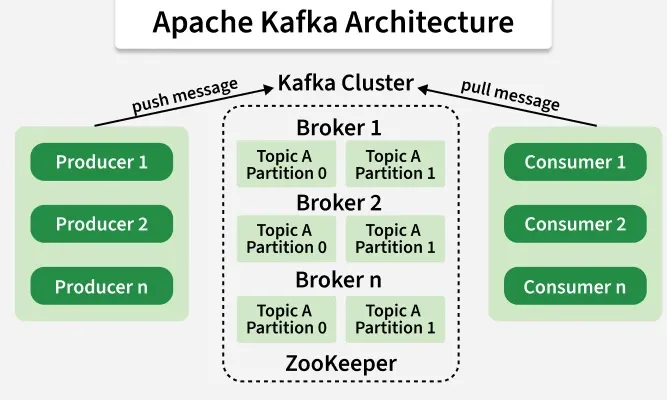
\includegraphics[width=0.65\linewidth]{images/architecture.png}
  {\fontsize{5}{6}\selectfont \url{https://www.geeksforgeeks.org/apache-kafka/kafka-architecture/}}

\end{frame}


\section{Componentes}

\begin{frame}\frametitle{Componentes - Commit log distribuido}
\begin{columns}
  \begin{column}{0.55\textwidth}
    \begin{itemize}
      \item \textbf{Estructura append-only}
      \begin{itemize}
        \item Escrituras secuenciales al final
        \item Inmutabilidad de eventos pasados
        \item Alta eficiencia de escritura y lectura
        \item Durabilidad de eventos configurable
      \end{itemize}

      \vspace{1em}

      \item \textbf{Offsets como punteros de lectura}
      \begin{itemize}
        \item Identificador único por mensaje en partición
        \item Orden secuencial de eventos por partición
        \item Permite lectura determinista por partición
        \item Checkpointing del progreso del consumidor
      \end{itemize}


    \end{itemize}
  \end{column}
  \begin{column}{0.45\textwidth}
    \centering
    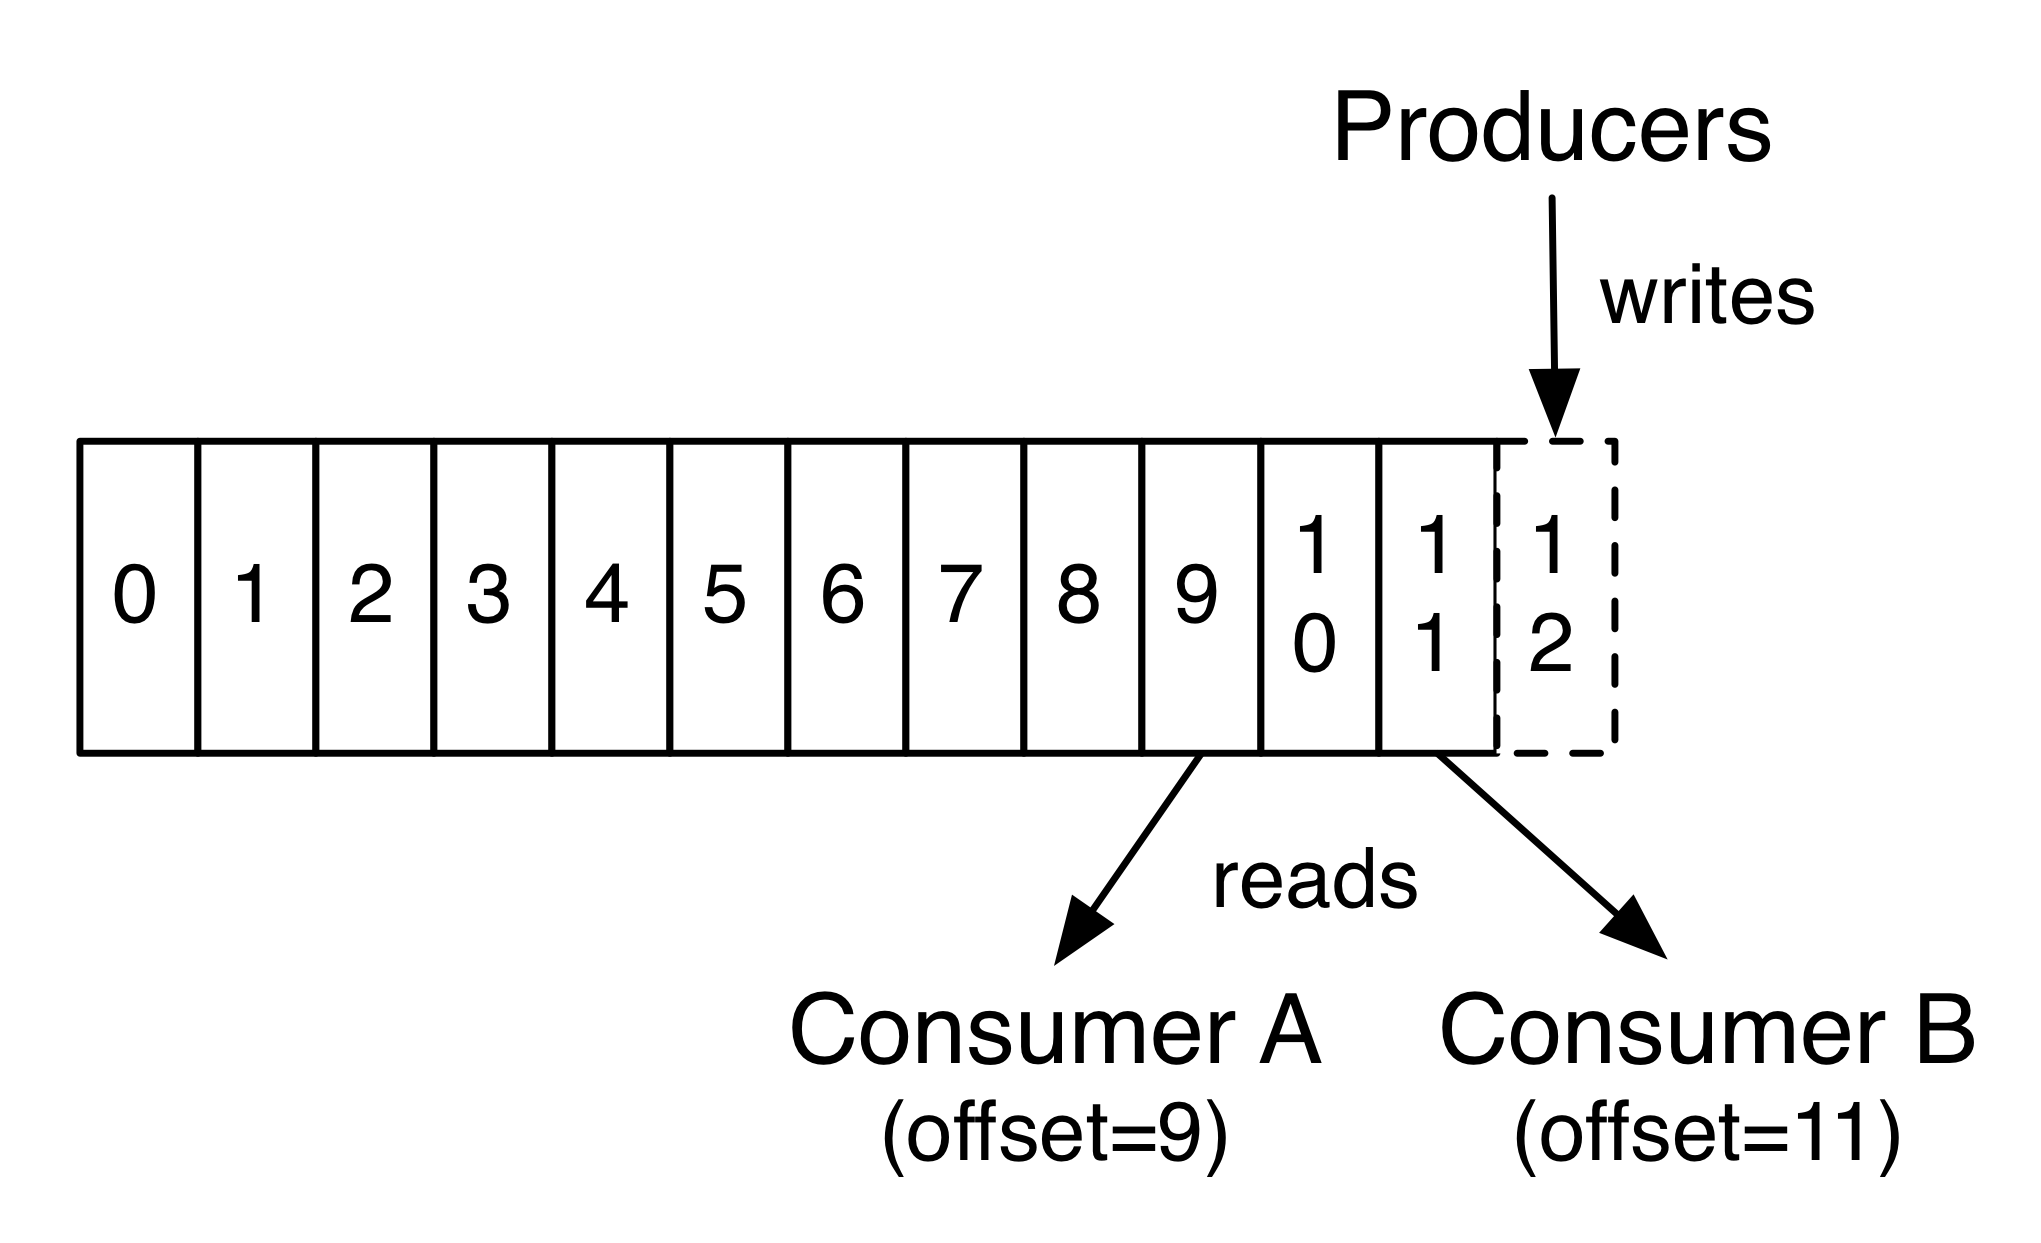
\includegraphics[width=0.8\linewidth]{images/consumer.png}

  \end{column}
\end{columns}
\end{frame}


\begin{frame}[fragile]\frametitle{Componentes - Mensajes}
\begin{itemize}
  \item \textbf{Estructura de un mensaje}
  \begin{itemize}
    \item \textbf{Key} (opcional) $\rightarrow$ ayuda a decidir partición y mantener orden por entidad
    \item \textbf{Value} $\rightarrow$ payload del mensaje en bytes
    \item \textbf{Timestamp} $\rightarrow$ marca temporal (por defecto del productor)
  \end{itemize}

  \vspace{1em}

  \item \textbf{Kafka no impone un formato específico}
  \begin{itemize}
    \item JSON (recomendado)
    \item Apache Avro para consistencia
  \end{itemize}
\end{itemize}
\end{frame}



\begin{frame}[fragile]\frametitle{Componentes - Mensajes}
\begin{itemize}
  \item Ejemplo de evento para gol en un partido
  \begin{shcode}
    // Kafka Key liga_2025_j27_001, Timestamp 2025-03-15T16:42:18Z
    {
      "schema_version": "1.0",
      "event_id": "3f7a2b9c-5d8e-4c1f-a6b3-9e4d2c1b5a7f",
      "event_time": "2025-03-15T16:42:18Z",
      "match_id": "liga_2025_j27_001",
      "event_type": "goal",
      "team_id": "real_madrid",
      "opponent_id": "barcelona",
      "scorer_id": "vinicius_jr",
      "assister_id": "modric",
      "minute": 67
    }
  \end{shcode}
\end{itemize}
\end{frame}


\begin{frame}\frametitle{Componentes - Esquema de un mensaje}
\begin{itemize}
  \item \textbf{Contrato que define la estructura de los datos}
  \begin{itemize}
    \item Plantilla que define qué campos tiene cada evento
    \item Facilita entendimiento entre productores y consumidores
    \item Evita errores $\rightarrow$ si falta un campo se detecta inmediatamente
  \end{itemize}

  \vspace{1em}

  \item \textbf{Ejemplo de esquema para evento de gol}
  \begin{itemize}
    \item \texttt{event\_id}: string
    \item \texttt{event\_time}: timestamp
    \item \texttt{match\_id}: string
    \item \texttt{event\_type}: string
    \item \texttt{scorer\_id}: string
    \item \texttt{assister\_id}: string
    \item \texttt{minute}: integer
  \end{itemize}

\end{itemize}
\end{frame}

\begin{frame}\frametitle{Componentes - Eficiencia con lotes y compresión}
\begin{itemize}
  \item \textbf{Lotes de mensajes}
  \begin{itemize}
    \item Colección de mensajes del mismo Topic y partición
    \item Reduce overhead de red y permite compresión
    \item En lugar de enviar 1 evento a la vez envía varios juntos
    \item Trade-off $\rightarrow$ lotes grandes pueden incrementar la latencia
  \end{itemize}

  \vspace{1em}

  \item \textbf{Compresión de datos}
  \begin{itemize}
    \item Ahorra espacio y velocidad de red
    \item Kafka soporta compresión configurable
    \item Existen varios algoritmos de compresión
  \end{itemize}
\end{itemize}
\end{frame}


\begin{frame}\frametitle{Componentes - Topics}
\begin{columns}
  \begin{column}{0.55\textwidth}
    \begin{itemize}
      \item \textbf{Canales lógicos donde se organizan los mensajes}
      \begin{itemize}
        \item Categoría de mensajes relacionados
        \item Organiza eventos por tipo o dominio
        \item Patrón común de nombrado $\rightarrow$ \texttt{dominio.subdominio.tipo.version}
      \end{itemize}

      \vspace{1em}

      \item \textbf{Configuraciones clave}
      \begin{itemize}
        \item Número particiones para paralelismo
        \item Factor de replicación para durabilidad
        \item Tiempo de retención de los mensajes
      \end{itemize}

      \vspace{1em}

      \item \textbf{Ejemplo \texttt{olympics.swimming.events.v1}}
    \end{itemize}
  \end{column}
  \begin{column}{0.5\textwidth}
    \centering
    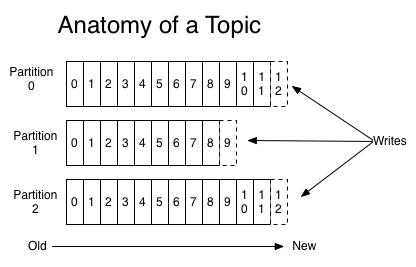
\includegraphics[width=0.8\linewidth]{images/partitions.png}
  \end{column}
\end{columns}
\end{frame}

\begin{frame}\frametitle{Componentes - Particiones}
\begin{columns}
  \begin{column}{0.55\textwidth}
    \begin{itemize}
      \item \textbf{Procesamiento en paralelo}
      \begin{itemize}
        \item Un Topic se divide en múltiples particiones
        \item Unidad de paralelismo y escalado horizontal
        \item Cada partición es un log ordenado independiente
        \item Es \textit{append-only} $\rightarrow$ se escribe al final
      \end{itemize}

      \vspace{1em}

      \item \textbf{Orden garantizado dentro de una partición}
      \begin{itemize}
        \item No garantiza orden en todo el Topic
        \item Key $\rightarrow$ misma partición
        \item Sin key $\rightarrow$ round-robin o sticky
      \end{itemize}
    \end{itemize}
  \end{column}
  \begin{column}{0.5\textwidth}
    \centering
    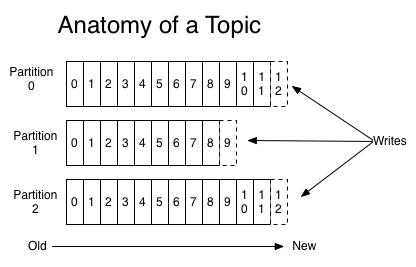
\includegraphics[width=0.8\linewidth]{images/partitions.png}
  \end{column}
\end{columns}
\end{frame}

\begin{frame}\frametitle{Componentes - Productores y consumidores}
\begin{itemize}
  \item \textbf{Productores}
  \begin{itemize}
    \item Escriben mensajes en Topics
    \item Balancean carga entre particiones
    \item Con \textit{key} garantizan orden por entidad en una partición
  \end{itemize}

  \vspace{1em}

  \item \textbf{Consumidores}
  \begin{itemize}
    \item Leen mensajes manteniendo orden dentro de cada partición
    \item Mantienen offsets con la posición del último mensaje leído
    \item Para recuperación tras fallo reinician desde el último offset guardado
  \end{itemize}
\end{itemize}
\end{frame}


\begin{frame}\frametitle{Componentes - Offsets}
\begin{columns}
  \begin{column}{0.58\textwidth}
    \begin{itemize}
      \item \textbf{Marcadores de lectura en partición}
      \begin{itemize}
        \item Permite recordar qué eventos se han procesado
        \item Como un marcador en un libro
      \end{itemize}

      \vspace{1em}

      \item \textbf{Ejemplo práctico de uso de offsets}
      \begin{itemize}
        \item Se disponen 1000 eventos GPS
        \item La lectura se cae en el evento 750
        \item Al reiniciar se continúa desde el 751
      \end{itemize}

      \vspace{1em}

      \item \textbf{Commit automático vs manual}
      \begin{itemize}
        \item En \textit{Auto} $\rightarrow$ Guarda el offset automáticamente
        \item En \textit{Manual} $\rightarrow$ Tú decides cuándo guardarlo
      \end{itemize}
    \end{itemize}
  \end{column}
  \begin{column}{0.42\textwidth}
    \centering
    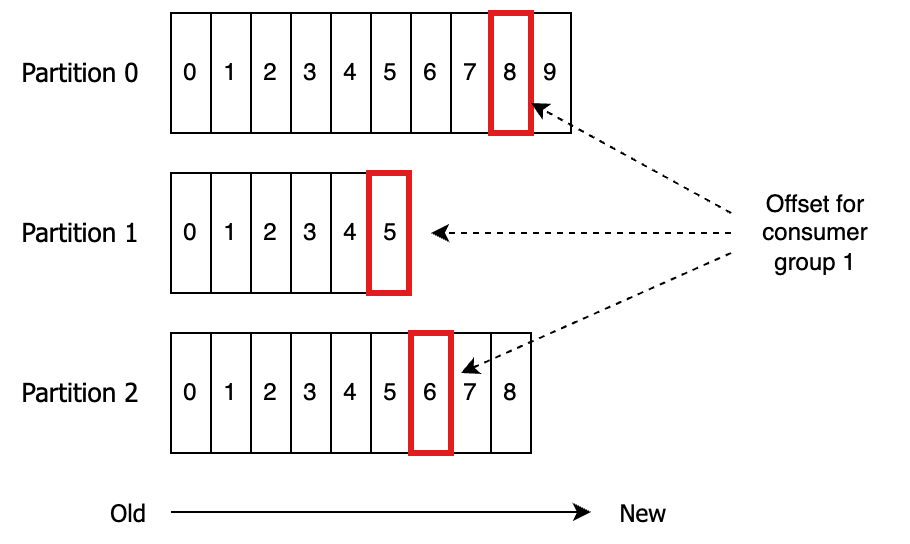
\includegraphics[width=0.95\linewidth]{images/offset.png}
  \end{column}
\end{columns}
\end{frame}

\begin{frame}\frametitle{Componentes - Lag del consumidor}
\begin{itemize}
  \item \textbf{Indica qué tan atrasado está el consumidor}
  \begin{itemize}
    \item Diferencia entre ultimo offset disponible y offset del consumidor
    \item End Offset=1000, Current Offset=750 $\rightarrow$ Lag=250 mensajes
  \end{itemize}

  \vspace{1em}
  \vspace{1em}

  \item \textbf{Importancia de monitorear el lag}
  \begin{itemize}
    \item Lag alto $\rightarrow$ consumidor lento o problemas de procesamiento
    \item Lag creciente $\rightarrow$ consumidor no puede mantener el ritmo
    \item Alertar cuando supera umbrales críticos
  \end{itemize}
\end{itemize}
\end{frame}

\begin{frame}\frametitle{Componentes - Distribución en consumidores}
\begin{itemize}
  \item \textbf{Un Topic puede ser leído por múltiples consumidores}

  \vspace{1em}

  \item \textbf{Mismo grupo de consumidores}
  \begin{itemize}
    \item Múltiples consumidores procesando en paralelo un Topic
    \item Si un consumidor procesa rápido, reduce el lag del grupo
    \item Si un consumidor falla, otros continúan
    \item Ejemplo $\rightarrow$ 3 consumidores procesando eventos GPS
  \end{itemize}

  \vspace{1em}

  \item \textbf{Único consumidor (distinto grupo)}
  \begin{itemize}
    \item Aplicaciones independientes
    \item Ejemplo $\rightarrow$ Dashboard + Análisis ML + DB histórica
  \end{itemize}
\end{itemize}
\end{frame}

\begin{frame}\frametitle{Componentes - Grupos de consumidores}
\begin{columns}
  \begin{column}{0.55\textwidth}
    \begin{itemize}
      \item \textbf{Permite paralelizar la lectura de un Topic}
      \begin{itemize}
        \item Escalabilidad horizontal de consumidores
        \item Consumidores agrupados por \texttt{group\_id}
        \item Paraleliza lectura dentro de un Topic
      \end{itemize}

      \vspace{1em}

      \item \textbf{Los mensajes se distribuyen en particiones}
      \begin{itemize}
        \item Dentro del grupo cada partición la lee un solo consumidor a la vez
        \item Para rendimiento máximo de lectura $\rightarrow$ particiones $\approx$ consumidores (en el grupo)
      \end{itemize}

      \vspace{1em}

      \item \textbf{Si un consumidor falla los restantes se reparten sus particiones}
    \end{itemize}
  \end{column}
  \begin{column}{0.45\textwidth}
    \centering
    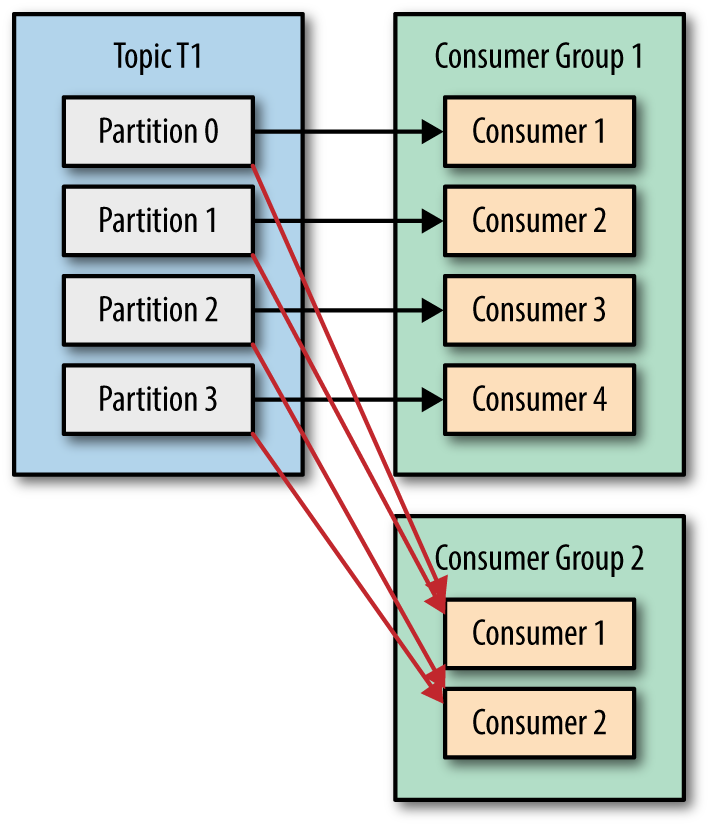
\includegraphics[width=0.7\linewidth]{images/consumer_group.png}
  \end{column}
\end{columns}
\end{frame}


\begin{frame}\frametitle{Componentes - Rebalance de grupos}
\begin{itemize}
  \item \textbf{Reasignación automática de particiones}
  \begin{itemize}
    \item Se activa cuando un consumidor se une, sale o falla
    \item Las particiones se redistribuyen entre consumidores activos
  \end{itemize}

  \vspace{1em}

  \item \textbf{Impacto durante el rebalance}
  \begin{itemize}
    \item El grupo deja de consumir temporalmente
    \item Puede causar duplicados si no se commitean offsets antes
    \item Tiempo de pausa depende del tamaño del grupo
  \end{itemize}

  \vspace{1em}

  \item \textbf{Varias estrategias de asignación}
  \begin{itemize}
    \item Range, Round-robin, Sticky
  \end{itemize}
\end{itemize}
\end{frame}


\section{Infraestructura}


\begin{frame}\frametitle{Infraestructura - Brokers y Clúster}
\begin{itemize}
  \item \textbf{Broker}
  \begin{itemize}
    \item Almacena particiones asignadas
    \item Es un servidor individual (nodo) del clúster
    \item Tienen un identificador único
  \end{itemize}

  \vspace{1em}

  \item \textbf{Clúster}
  \begin{itemize}
    \item Conjunto de brokers coordinados
    \item Un broker actúa como controlador
    \item Distribución de particiones entre brokers
  \end{itemize}

  \vspace{1em}

  \item \textbf{Permite escalabilidad y alta disponibilidad}
\end{itemize}
\end{frame}


\begin{frame}\frametitle{Infraestructura - Replicación y tolerancia a fallos}
\begin{columns}
  \begin{column}{0.45\textwidth}
    \begin{itemize}
      \item \textbf{Modelo líder-seguidor}
      \begin{itemize}
        \item Líder maneja lecturas y escrituras
        \item Seguidores copian log del líder
      \end{itemize}

      \vspace{1em}

      \item \textbf{In-Sync Replicas (ISR)}
      \begin{itemize}
        \item Réplicas sincronizadas con el líder
        \item Pueden ser elegidas como líder
      \end{itemize}

      \vspace{1em}

      \item \textbf{Si el líder falla se elige otro}
      \begin{itemize}
        \item Nuevo líder es un seguidor en ISR
        \item El sistema sigue funcionando sin pérdida
      \end{itemize}
    \end{itemize}
  \end{column}
  \begin{column}{0.5\textwidth}
    \centering
    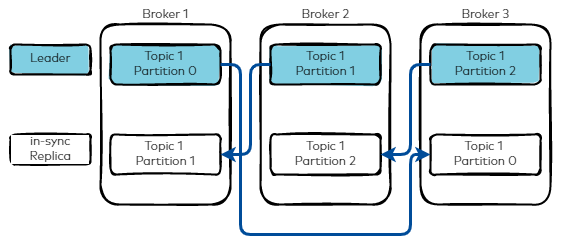
\includegraphics[width=\linewidth]{images/replication.png}
  \end{column}
\end{columns}
\end{frame}

\begin{frame}\frametitle{Infraestructura - Garantías de escritura}
\begin{itemize}
  \item \textbf{Acknowledgment (ack)}
  \begin{itemize}
    \item Recibido por el productor
    \item Brokers confirman mensajes recibidos
  \end{itemize}

  \vspace{1em}

  \item \textbf{Tipos de acknowledgment}
  \begin{itemize}
    \item \texttt{acks=0} $\rightarrow$ sin confirmación
    \item \texttt{acks=1} $\rightarrow$ líder confirma
    \item \texttt{acks=all} $\rightarrow$ todas las ISR confirman
  \end{itemize}
\end{itemize}
\end{frame}

\begin{frame}\frametitle{Infraestructura - Garantías de entrega}
\begin{itemize}
  \item \textbf{At-most-once}
  \begin{itemize}
    \item El dato puede perderse pero no se duplica
    \item Cuando velocidad es más importante que completitud
    \item Ejemplo $\rightarrow$ Sensor GPS falla, pierdes una posición
  \end{itemize}

  \vspace{1em}

  \item \textbf{At-least-once} - Opción más común
  \begin{itemize}
    \item El dato llega pero puede duplicarse
    \item Garantiza que no se pierden eventos
    \item Ejemplo $\rightarrow$ El mismo gol aparece dos veces en tu sistema

  \end{itemize}

  \vspace{1em}

  \item \textbf{Exactly-once}
  \begin{itemize}
    \item El dato se procesa una vez
    \item Kafka lo soporta pero requiere configuración avanzada
  \end{itemize}
\end{itemize}
\end{frame}

\begin{frame}\frametitle{Infraestructura - Durabilidad de datos}
\begin{itemize}
  \item \textbf{Durabilidad es no perder datos}
  
  \vspace{1em}

  \item \textbf{Tres pilares para garantizar durabilidad}
  \begin{itemize}
    \item Producers esperan confirmación del broker
    \item Múltiples copias en ISR
    \item Datos escritos a disco
  \end{itemize}

  \vspace{1em}

  \item \textbf{Mayor durabilidad implica mayor latencia}
\end{itemize}
\end{frame}

\begin{frame}\frametitle{Infraestructura - Coordinación del clúster}
\begin{columns}
  \begin{column}{0.58\textwidth}
    \begin{itemize}
      \item \textbf{Zookeeper (legacy)}
      \begin{itemize}
        \item Almacena metadatos del clúster y coordina elección de líderes
        \item Ensemble con número impar de nodos (3, 5, 7)
        \item Requiere gestión adicional de infraestructura
      \end{itemize}

      \vspace{1em}

      \item \textbf{KRaft (Kafka 3.0+)}
      \begin{itemize}
        \item Gestiona metadatos y líderes sin Zookeeper
        \item Protocolo Raft para consenso y elección de líderes
        \item Menos complejidad y arranque más rápido
      \end{itemize}

      \vspace{1em}

      \item \textbf{Se recomienda KRaft para nuevos clústeres}
    \end{itemize}
  \end{column}
  \begin{column}{0.42\textwidth}
    \centering
    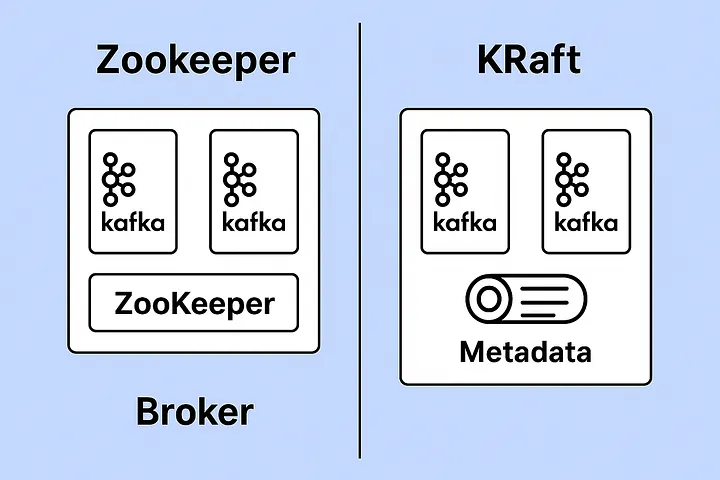
\includegraphics[width=0.95\linewidth]{images/zookeeper_kraft.png}
  \end{column}
\end{columns}
\end{frame}

\begin{frame}\frametitle{Infraestructura - Dimensionamiento de particiones}
\begin{itemize}
  \item \textbf{Regla práctica}
  \begin{itemize}
    \item Particiones $\approx$ \textbf{throughput deseado} / \textbf{velocidad del consumidor}
    \item Ejemplo $\rightarrow$ 1 GB/s / 50 MB/s $\approx$ 20 particiones
  \end{itemize}
  \vspace{1em}

  \item \textbf{Consideraciones}
  \begin{itemize}
    \item Se pueden aumentar, pero no disminuir
    \item Más particiones $\rightarrow$ más concurrencia
    \item Demasiadas $\rightarrow$ mayor uso de memoria y coste de coordinación
  \end{itemize}
\end{itemize}
\end{frame}

\begin{frame}\frametitle{Infraestructura - Políticas de retención}
\begin{itemize}
  \item \textbf{Retención por tiempo}
  \begin{itemize}
    \item Se borran segmentos cuando el último mensaje supera la edad límite
    \item Ejemplo $\rightarrow$ conservar datos de un partido durante 7 días
  \end{itemize}

  \vspace{1em}

  \item \textbf{Retención por tamaño}
  \begin{itemize}
    \item Útil para evitar llenar el disco con flujos impredecibles
    \item Ejemplo $\rightarrow$ máximo 1GB por partición
  \end{itemize}

  \vspace{1em}

  \item \textbf{Log compaction}
  \begin{itemize}
    \item Mantiene el último valor por clave
    \item Elimina versiones antiguas de la misma clave
    \item Ejemplo $\rightarrow$ Mantener última posición GPS de cada jugador
  \end{itemize}
\end{itemize}
\end{frame}

\section{Ejemplos}

\begin{frame}[fragile]\frametitle{Ejemplos - Kafka con Docker}
\begin{itemize}
  \item \textbf{Kafka 4.1+ incluye KRaft (sin Zookeeper)}
  \begin{itemize}
    \item Arranque rápido con un solo contenedor
    \item Ideal para desarrollo y pruebas locales
  \end{itemize}

  \vspace{1em}

  \item \textbf{Comando para lanzar Kafka localmente}
  \begin{itemize}
    \item Puerto 9092 expuesto para productores y consumidores
    \item Broker disponible en \texttt{localhost:9092}
  \end{itemize}
\end{itemize}

\vspace{1em}

\begin{shellbox}
\begin{shcode}
docker run -p 9092:9092 apache/kafka:4.1.1
\end{shcode}
\end{shellbox}


\end{frame}


\begin{frame}[fragile]\frametitle{Ejemplos - Kafka con Docker Avanzado}
\begin{shellbox}
\begin{shcode}
docker run -p 9092:9092 \
  -e KAFKA_HEAP_OPTS="-Xmx1G -Xms1G" \           # Memoria JVM
  -e KAFKA_LOG_RETENTION_HOURS=168 \             # Retencion 7 dias
  -e KAFKA_NUM_PARTITIONS=3 \                    # Particiones defecto
  -e KAFKA_DEFAULT_REPLICATION_FACTOR=1 \        # Factor replicacion
  -e KAFKA_COMPRESSION_TYPE=gzip \               # Compresion
  apache/kafka:4.1.1
\end{shcode}
\end{shellbox}
\end{frame}


\begin{frame}[fragile]\frametitle{Ejemplos - Kafka con Docker Compose}
\begin{shcode}
    services:
      kafka:
        image: apache/kafka:4.1.1
        ports:
          - "9092:9092"
        volumes:
          - kafka-data:/var/lib/kafka/data    # Persistencia
        environment:
          KAFKA_HEAP_OPTS: "-Xmx1G -Xms1G"    # Memoria JVM
          KAFKA_LOG_RETENTION_HOURS: 168      # Retencion 7 dias
          KAFKA_NUM_PARTITIONS: 3             # Particiones defecto
          KAFKA_DEFAULT_REPLICATION_FACTOR: 1 # Factor replicacion
          KAFKA_COMPRESSION_TYPE: gzip        # Compresion
\end{shcode}
\end{frame}


\begin{frame}\frametitle{Kafka con Python}
\begin{itemize}
    \item \textbf{Librería \texttt{kafka-python} para casos de uso sencillos}
    \begin{itemize}
        \item Cliente básico de Kafka para Python
        \item Soporte completo para Producer y Consumer
    \end{itemize}
    \vspace{0.3cm}
    \item \textbf{Componentes principales}
    \begin{itemize}
        \item \texttt{KafkaProducer}: Envía mensajes a topics
        \item \texttt{KafkaConsumer}: Lee mensajes de topics
        \item \texttt{KafkaAdminClient}: Gestión de topics y configuración
    \end{itemize}
    \vspace{0.3cm}
    \item \textbf{Librería \texttt{confluent-kafka} para producción y alto rendimiento}
\end{itemize}
\end{frame}


\begin{frame}[fragile]\frametitle{Ejemplos - Producer básico}
\begin{code}
\begin{python3code}
from kafka import KafkaProducer
import json
import random
import time

producer = KafkaProducer(
    bootstrap_servers=['localhost:9092'],
    value_serializer=lambda v: json.dumps(v).encode('utf-8')
)

for i in range(100):
    message = {'id': i, 'value': random.randint(1, 100)}
    producer.send('random.numbers.v1', value=message)
    time.sleep(1)

producer.close()
\end{python3code}
\end{code}
\end{frame}


\begin{frame}[fragile]\frametitle{Ejemplos - Producer avanzado}
\begin{code}
\begin{python3code}
producer = KafkaProducer(
    bootstrap_servers=['localhost:9092'],
    value_serializer=lambda v: json.dumps(v).encode('utf-8'),

    # Garantías de entrega
    acks='all',              # 0, 1, o 'all'
    retries=3,               # reintentos
    enable_idempotence=True, # exactly-once

    # Rendimiento
    compression_type='gzip', # gzip, snappy, lz4, zstd
    batch_size=16384,        # tamaño lote (bytes)
    linger_ms=10             # espera antes de enviar
)
\end{python3code}
\end{code}
\end{frame}


\begin{frame}[fragile]\frametitle{Ejemplos - Consumer básico}
\begin{code}
\begin{python3code}
from kafka import KafkaConsumer
import json

consumer = KafkaConsumer(
    'random.numbers.v1',
    bootstrap_servers=['localhost:9092'],
    auto_offset_reset='latest',
    value_deserializer=lambda m: json.loads(m.decode('utf-8'))
)

print("Listening for messages...")

for message in consumer:
    data = message.value
    print(f"Received: ID={data['id']}, Value={data['value']}")
\end{python3code}
\end{code}
\end{frame}


\begin{frame}[fragile]\frametitle{Ejemplos - Consumer avanzado}
\begin{code}
\begin{python3code}
consumer = KafkaConsumer(
    'random.numbers.v1',
    bootstrap_servers=['localhost:9092'],

    # Deserialización de mensajes
    key_deserializer=lambda k: k.decode('utf-8') if k else None,
    value_deserializer=lambda m: json.loads(m.decode('utf-8')),

    # Grupo de consumidores
    group_id='my-consumer-group',

    # Gestión de offsets
    auto_offset_reset='latest',    # earliest, latest, none
)
\end{python3code}
\end{code}
\end{frame}


\begin{frame}\frametitle{Conclusiones}
\begin{itemize}
  \item \textbf{Kafka como hub central de datos deportivos}
  \begin{itemize}
    \item Reduce complejidad y fragilidad frente a integraciones P2P
    \item Hub central para datos deportivos en tiempo real
  \end{itemize}

  \vspace{0.5em}

  \item \textbf{Kafka es un commit log distribuido}
  \begin{itemize}
    \item Persistencia y retención $\rightarrow$ replay y múltiples consumidores
    \item Topics/particiones $\rightarrow$ orden por partición y paralelismo
    \item Offsets $\rightarrow$ control del progreso y recuperación ante fallos
  \end{itemize}

  \vspace{0.5em}

  \item \textbf{Operación y escalado requieren diseño}
  \begin{itemize}
    \item Replicación líder/seguidores, dimensionamiento de particiones
    \item Políticas de retención según tipo de dato deportivo
    \item Configuración apropiada para garantías de entrega
  \end{itemize}
\end{itemize}
\end{frame}

\end{document}
